% ============================================================
%  Section V — Preliminary Findings and Insights
%  Drop-in replacement for the existing Section V.
%  Requires packages: booktabs, multirow, graphicx, subcaption, pgfplots, xcolor
%  Table numbers continue from Table III (planner primitives).
%  Adjust \label{tab:...} cross-references to match your numbering.
% ============================================================

\section{Preliminary Findings and Insights}

\subsection{Velocity-Control Policy Evaluation}

Initial fine-tuning experiments employed a velocity-control action representation in which
the policy directly predicted joint velocity commands.
The resulting policy demonstrated evidence of language grounding and task understanding,
consistently approaching the correct coloured block in response to the provided language
instruction.

Despite this promising behaviour, reliable manipulation was not achieved.
Quantitative evaluation confirmed this: the \texttt{vel\_pickplace\_99999} checkpoint
achieved 0\% trial-level success across all 40 evaluated trials
(four tasks, 10~trials each) and a block-lifted rate of 0\% throughout
(Table~\ref{tab:success}).
Mean gripper close step of 762 and 940 for the red-far and red-near tasks respectively
indicates that the gripper consistently failed to close during the approach phase,
instead remaining open for the full 600-step episode.
The policy frequently contacted the block through arm translation rather than a
controlled grasp, displacing it unpredictably.

These experiments provided an important insight: the model had learned the relationship
between visual observations, language instructions, and task objectives, but struggled to
translate this understanding into precise manipulation actions.
This observation motivated further investigation into train--inference mismatches and
ultimately led to the transition towards position-control actions.

\subsection{Analysis of Train--Inference Mismatches}

A significant portion of the project involved identifying discrepancies between
demonstration generation and policy deployment.
Several train--inference mismatches were discovered during evaluation and were found to
have a substantial impact on policy performance.

The first major issue involved incorrect action targets during dataset generation.
Actions were initially recorded as small position deltas derived from velocity commands,
resulting in target magnitudes of approximately 0.001~rad after downsampling.
The trained policy consequently produced negligible arm motion during inference,
with mean action magnitudes of $\sim$0.001~rad across all joints
compared to the expected 0.05--0.3~rad range.
Correcting the action targets to represent the desired joint configuration at the
subsequent timestep resolved this issue and enabled meaningful motion generation.

Further investigation identified a grasp alignment error in which the gripper
consistently stopped approximately 2--3~cm above the block centre during demonstration
collection, due to a descent tolerance of 0.025~m.
This error was confirmed diagnostically via per-step grasp position logging showing
consistent $z$-errors of $+28$--$30$~mm.
Reducing the descent target to $z_\text{block} - 0.010$~m with tolerance 0.010~m
corrected the grip site to within 1~mm of block centre.

Additional deployment-specific issues were identified:
\begin{itemize}
    \item \emph{Gripper initialisation mismatch:} \texttt{mj\_resetDataKeyframe} resets
    joint positions but not control signals, causing the policy to observe
    gripper\_norm~$\approx 0.65$ at step~0 rather than 0.0 as seen during training.
    This caused the policy to immediately enter carry mode, oscillating between two arm
    configurations for the full 600-step episode.
    Fixed by explicitly setting \texttt{ctrl[gripper] = OPEN} after keyframe reset.

    \item \emph{Gripper hysteresis:} The flow-matching denoising process occasionally
    produced close--open--close patterns within a single 10-step action chunk,
    causing the block to escape mid-carry.
    Fixed by latching the gripper closed once a grasp is detected
    (gripper\_norm~$> 0.5$), releasing only on a clear placement signal
    (gripper\_norm~$< 0.2$).
\end{itemize}

Addressing these mismatches highlighted a broader principle: the
train--inference boundary in VLA adaptation is as important as the
training configuration itself.
Fig.~\ref{fig:state_mismatch} illustrates the gripper state divergence
over an episode before and after the initialisation fix was applied.

\begin{figure}[t]
    \centering
    
\includegraphics[width=\columnwidth]{%
        /home/robotlab/Desktop/saniya_ws/pi0.5_mujoco/data/baxter/plots/04_state_mismatch.png}
    \caption{Gripper state (normalised) observed by the policy over a 150-step episode,
    illustrating the initialisation mismatch: without the fix (dashed), the policy
    perceives gripper\_norm~$\approx 0.65$ at step~0 and immediately enters carry mode.
    After the fix (solid), the policy correctly begins with gripper\_norm~$= 0.0$
    and executes the intended approach--grasp sequence.}
    \label{fig:state_mismatch}
\end{figure}

\subsection{Position-Control Policy Evaluation}

To address the limitations observed in velocity-control experiments, the action
representation was redesigned to predict target joint positions rather than joint
velocities.
Under this formulation, a proportional controller converts predicted targets into
executable velocity commands:
\begin{equation}
    v = \operatorname{clip}\!\left(K_P\,(q_{\mathrm{target}} - q),\;
        -v_{\max},\; v_{\max}\right)
    \label{eq:pctrl}
\end{equation}
with $K_P = 40$ and $v_{\max} = 1.5$~rad/s.
This separates the \emph{where} (learned by the policy) from the \emph{how fast}
(handled by the controller), substantially simplifying the learning problem.

The resulting policies demonstrated noticeably improved manipulation behaviour,
generating smoother trajectories, more stable object approach motions, and
more consistent grasp attempts.
The \texttt{pos\_run3\_199999} checkpoint achieved 20\% trial-level success
(12/60 trials) compared to 0\% for the velocity-control baseline,
with the block-lifted rate rising from 0\% to 13--30\% across tasks that
had previously shown no successful manipulation.
Position-control policies were therefore adopted as the standard representation
for all subsequent training runs.

\subsection{Checkpoint Comparison and Policy Evolution}

Five policy checkpoints were evaluated across the full six-task protocol
(10 trials per task, 60 trials per checkpoint, except the velocity-control checkpoint
which covers four tasks only).
The checkpoints represent successive design iterations:
\texttt{pi05\_base} (zero-shot), \texttt{vel\_pickplace\_99999} (100k steps,
velocity control), \texttt{pos\_run3\_199999} (200k steps, position control),
\texttt{pos\_v2\_499999} (500k steps, native 10~Hz recording, 11-dim state), and
\texttt{pos\_v3} (200k warm-start fine-tuning steps from \texttt{pos\_v2},
augmented near-side demonstrations).

\subsubsection{Trial-Level Success Rate}

Table~\ref{tab:success} reports per-task trial-level success rates across all
checkpoints.
A trial is successful if the specified block reaches the correct side of the
workspace divider ($x > 0.70$~m for far; $x < 0.66$~m for near).

% ------------------------------------------------------------------
%  TABLE: Per-task trial-level success rate
% ------------------------------------------------------------------
\begin{table*}[t]
\centering
\caption{Per-task trial-level success rate (successes / 10 trials).
$\dagger$: green-block tasks were not in the velocity-control training set.
Highest value per task shown in \textbf{bold}.}
\label{tab:success}
\setlength{\tabcolsep}{5pt}
\small
\begin{tabular}{@{}llccccc@{}}
\toprule
\textbf{Task} & \textbf{Instruction} &
    \textbf{pi05\_base} &
    \textbf{vel 100k} &
    \textbf{pos 200k} &
    \textbf{pos\_v2 500k} &
    \textbf{pos\_v3} \\
\midrule
T0 & Move red block $\to$ far   & 7/10 & 0/10 & 1/10 & 6/10 & \textbf{9/10} \\
T1 & Move red block $\to$ near  & 2/10 & 0/10 & 2/10 & 4/10 & \textbf{4/10} \\
T2 & Move blue block $\to$ far  & 0/10 & 0/10 & \textbf{8/10} & 7/10 & \textbf{9/10} \\
T3 & Move blue block $\to$ near & 0/10 & 0/10 & 0/10 & \textbf{5/10} & 4/10 \\
T4 & Move green block $\to$ far & 0/10 & $-^\dagger$ & 1/10 & 2/10 & \textbf{0/10} \\
T5 & Move green block $\to$ near& 0/10 & $-^\dagger$ & 0/10 & 0/10 & \textbf{0/10} \\
\midrule
\multicolumn{2}{@{}l}{\textbf{Overall (trial-level)}} &
    9/60 (15\%) & 0/40 (0\%) & 12/60 (20\%) & 24/60 (40\%) & \textbf{26/60 (43\%)} \\
\multicolumn{2}{@{}l}{\quad Far-side average} &
    23\% & 0\% & 33\% & 50\% & \textbf{60\%} \\
\multicolumn{2}{@{}l}{\quad Near-side average} &
    7\% & 0\% & 13\% & 30\% & 27\% \\
\bottomrule
\end{tabular}
\end{table*}

Several findings emerge from Table~\ref{tab:success}.
First, the zero-shot \texttt{pi05\_base} baseline achieves a non-trivial 15\%
overall success rate (9/60 trials), with particularly strong performance on T0
(7/10, 70\% success).
This result --- which contrasts with the na\"{i}ve expectation that the pretrained
model would entirely fail on an unseen embodiment --- confirms that $\pi$0.5 retains
transferable manipulation priors, while also demonstrating that fine-tuning is
necessary for reliable multi-task performance.

Second, a consistent far-side advantage is observed across all fine-tuned
position-control checkpoints (far average: 20--60\%; near average: 7--30\%).
Near-side carry requires the arm to move inward toward the robot base, which
conflicts with the DLS null-space configuration and produces less consistent
training demonstrations.

Third, green-block tasks (T4, T5) represent a persistent failure mode across
all checkpoints, including \texttt{pos\_v3} which was explicitly augmented with
250 near-side green demonstrations per task.
The green block's position ($y = +0.05$~m toward the robot midline) requires
an arm configuration that approaches joint limits, and the \texttt{pos\_v3}
checkpoint shows \emph{regression} on T4 (1/10 $\to$ 0/10) relative to
\texttt{pos\_v2}, suggesting that the lower learning rate warm-start did not
provide sufficient gradient signal for this task.

\subsubsection{Manipulation Quality: Block-Lifted Rate}

Task success alone conflates true pick-and-place with accidental push success.
Table~\ref{tab:lifted} disaggregates these by reporting the block-lifted rate,
defined as the fraction of trials in which the block exceeded $z > 0.295$~m
(above table height of 0.260~m plus block half-height of 0.025~m),
confirming a genuine grasp-and-lift occurred.

% ------------------------------------------------------------------
%  TABLE: Block-lifted rate
% ------------------------------------------------------------------
\begin{table*}[t]
\centering
\caption{Block-lifted rate (\% of trials in which true pick-and-place was executed,
i.e.\ block\_z $> 0.295$~m during the episode).
The gap between this table and Table~\ref{tab:success} indicates push-based
rather than pick-based success. \textbf{Bold}: highest per task.}
\label{tab:lifted}
\setlength{\tabcolsep}{5pt}
\small
\begin{tabular}{@{}llccccc@{}}
\toprule
\textbf{Task} & \textbf{Instruction} &
    \textbf{pi05\_base} &
    \textbf{vel 100k} &
    \textbf{pos 200k} &
    \textbf{pos\_v2 500k} &
    \textbf{pos\_v3} \\
\midrule
T0 & Move red block $\to$ far   & 80\% & 0\% & 20\% & 70\% & \textbf{90\%} \\
T1 & Move red block $\to$ near  & 20\% & 0\% & 30\% & 50\% & \textbf{70\%} \\
T2 & Move blue block $\to$ far  & 0\%  & 0\% & 30\% & \textbf{90\%} & 80\% \\
T3 & Move blue block $\to$ near & 0\%  & 0\% & 30\% & \textbf{60\%} & \textbf{70\%} \\
T4 & Move green block $\to$ far & 0\%  & $-$ & 10\% & \textbf{30\%} & 0\% \\
T5 & Move green block $\to$ near& 0\%  & $-$ & 10\% & 0\% & 0\% \\
\midrule
\multicolumn{2}{@{}l}{\textbf{Mean lifted rate (all tasks)}} &
    17\% & 0\% & 22\% & \textbf{50\%} & 45\% \\
\bottomrule
\end{tabular}
\end{table*}

Comparing Tables~\ref{tab:success} and~\ref{tab:lifted} reveals an important
discrepancy for the \texttt{pos\_run3} checkpoint at T2 (blue $\to$ far):
8/10 task-success but only 30\% lift rate, indicating that the majority of
T2 successes were achieved through inadvertent pushing rather than controlled
pick-and-place.
Post-hoc grasp diagnostics confirmed a mean grasp error of
$(-155,\,-78,\,-2)$~mm for T2: the gripper closed 15.5~cm laterally displaced
from the block, and arm translation displaced the block to the far side.

By contrast, the \texttt{pos\_v2} and \texttt{pos\_v3} checkpoints achieve lift
rates substantially above their task-success rates for blue tasks (90\%, 80\%
lifted vs.\ 70\%, 90\% success), confirming that genuine pick-and-place is being
executed.
The \texttt{pos\_v3} checkpoint achieves the highest average lift rates for red
tasks (90\% and 70\% for T0 and T1 respectively), indicating reliable grasp
execution for the red block despite the overall modest improvement in task success.

\subsubsection{Direction Accuracy}

Table~\ref{tab:direction} reports the fraction of trials in which the block was
displaced in the correct direction (positive $x$-displacement for far tasks,
negative for near tasks), regardless of whether the success threshold was crossed.
This metric measures task understanding independently of execution precision.

% ------------------------------------------------------------------
%  TABLE: Direction accuracy + mean displacement
% ------------------------------------------------------------------
\begin{table*}[t]
\centering
\caption{Direction accuracy (\% of trials with correct-direction block displacement)
and mean signed block displacement (m; positive = toward far side).
Direction accuracy measures task understanding; displacement quantifies
proximity to success for near-miss trials.}
\label{tab:direction}
\setlength{\tabcolsep}{4.5pt}
\small
\begin{tabular}{@{}llcccccccccc@{}}
\toprule
& & \multicolumn{5}{c}{\textbf{Direction Accuracy (\%)}} &
    \multicolumn{5}{c}{\textbf{Mean Displacement (m)}} \\
\cmidrule(lr){3-7}\cmidrule(lr){8-12}
\textbf{Task} & \textbf{Instruction} &
    Base & Vel & Pos & V2 & V3 &
    Base & Vel & Pos & V2 & V3 \\
\midrule
T0 & Red $\to$ far   & 100 & 0  & 50  & 100 & 100 & $+0.127$ & $+0.000$ & $+0.022$ & $+0.116$ & $+0.159$ \\
T1 & Red $\to$ near  & 40  & 0  & 50  & 40  & 40  & $-0.015$ & $+0.000$ & $-0.020$ & $-0.031$ & $-0.022$ \\
T2 & Blue $\to$ far  & 20  & 0  & 80  & 100 & 90  & $+0.003$ & $+0.000$ & $+0.128$ & $+0.126$ & $+0.121$ \\
T3 & Blue $\to$ near & 0   & 0  & 0   & 50  & 40  & $+0.001$ & $+0.000$ & $+0.054$ & $-0.056$ & $-0.024$ \\
T4 & Green $\to$ far & 10  & $-$& 50  & 80  & 0   & $-0.000$ & $-$      & $+0.022$ & $+0.063$ & $+0.000$ \\
T5 & Green $\to$ near& 0   & $-$& 0   & 0   & 0   & $+0.000$ & $-$      & $+0.033$ & $+0.005$ & $+0.000$ \\
\bottomrule
\end{tabular}
\end{table*}

Direction accuracy reveals task understanding that is not captured by binary
success metrics.
The \texttt{pos\_v2} checkpoint achieves 100\% direction accuracy on both T0
and T2 and 80\% on T4, yet its task success on T4 remains only 20\%.
This confirms that the policy understands which direction to move for these tasks
but lacks the precision to cross the success threshold.
By contrast, the \texttt{pos\_v3} checkpoint regresses to 0\% direction
accuracy on T4 (green $\to$ far), consistent with the collapsed prediction
behaviour (arm hovering at pregrasp for 600 steps) observed during diagnostic
rollouts.

\subsubsection{Training Metrics and Loss--Performance Relationship}

Table~\ref{tab:training} summarises the training configurations and final
loss values for all fine-tuned checkpoints.

% ------------------------------------------------------------------
%  TABLE: Training metrics
% ------------------------------------------------------------------
\begin{table}[t]
\centering
\caption{Training configuration and final metrics for each fine-tuned checkpoint.
All runs use AdamW optimiser, cosine LR decay, LoRA rank~16 on PaliGemma-2B
and Gemma-300M action expert.}
\label{tab:training}
\small
\begin{tabular}{@{}lccccc@{}}
\toprule
\textbf{Config} & \textbf{Steps} & \textbf{Peak LR} & \textbf{Data} &
    \textbf{State} & \textbf{Final Loss} \\
\midrule
vel 100k   & 100k & $2\!\times\!10^{-4}$ & 400 ep & 8-dim & $-$ \\
pos 200k   & 200k & $2\!\times\!10^{-4}$ & 600 ep & 8-dim & 0.008--0.015 \\
pos\_v2 500k & 500k & $2\!\times\!10^{-4}$ & 600 ep & 11-dim & 0.004 \\
pos\_v3    & $+$200k & $5\!\times\!10^{-5}$ & $\sim$950 ep & 11-dim & $<$0.004 \\
\bottomrule
\end{tabular}
\end{table}

A key finding is that lower training loss does not correspond monotonically to
improved task performance.
The \texttt{pos\_v2} checkpoint achieves a final loss of 0.004 --- substantially
lower than \texttt{pos\_run3} (0.008--0.015) --- yet achieves only marginal
improvement in overall task success (40\% vs.\ 20\%).
More strikingly, \texttt{pos\_v2} achieves fewer successes than
\texttt{pos\_run3} on T2 (7/10 vs.\ 8/10) despite training 2.5$\times$ longer.
These observations indicate that the primary bottleneck is not optimisation
depth but rather the quality of training data (demonstration frequency,
state representation, and grasp precision).
The introduction of native 10~Hz demonstration recording and end-effector
Cartesian coordinates in \texttt{pos\_v2} had a greater qualitative effect
on lifting behaviour (mean lifted rate 50\% vs.\ 22\%) than on raw task success.

\subsubsection{Failure Mode Analysis}

Table~\ref{tab:failures} summarises the per-task failure modes identified
through diagnostic logging of grasp position errors, action magnitudes,
and block trajectories for the \texttt{pos\_run3} checkpoint.

% ------------------------------------------------------------------
%  TABLE: Failure modes
% ------------------------------------------------------------------
\begin{table}[t]
\centering
\caption{Per-task failure modes and diagnostic measurements for
\texttt{pos\_run3\_199999}.
Grasp error $(e_x, e_y, e_z)$ is the vector from gripper centre to
block centre at the moment of gripper close.}
\label{tab:failures}
\small
\begin{tabular}{@{}llp{3.8cm}@{}}
\toprule
\textbf{Task} & \textbf{Primary Failure} & \textbf{Diagnostic} \\
\midrule
T0 (red far)  & Placement 1.5~cm short   & Grasp error $(-3,-2,-3)$~mm; correct carry direction; oscillation post-grasp \\
T1 (red near) & Mid-chunk grip release   & Grasp fired twice at steps 27 \& 29; block displaced 8~mm $x$, 12~mm $y$ during oscillation \\
T2 (blue far) & Push, not pick           & Grasp error $(-155,-78,-2)$~mm; accidental far-side displacement \\
T3 (blue near)& Grasp miss               & Grasp error $(-51,-22,+6)$~mm; gripper closed on air \\
T4 (green far)& Collapsed prediction     & No grasp event in 600 steps; arm hovered at pregrasp (q0$\approx$0.85) \\
T5 (green near)& Z-height error          & Grasp error $(-0.3,+23,+29)$~mm; grip site 29~mm above block centre \\
\bottomrule
\end{tabular}
\end{table}

The failure modes in Table~\ref{tab:failures} fall into three distinct
categories.
\emph{Precision failures} (T0, T3, T5) indicate that the policy has learned
the correct arm trajectory structure but lacks fine-grained spatial accuracy
at the grasp moment; these are addressable through additional training data
with greater block position randomisation.
\emph{Temporal instability} (T1) results from the flow-matching diffusion
process producing locally inconsistent action sequences within a chunk;
the gripper latch fix described in Section~III-G resolves this at inference
time without retraining.
\emph{Representational failures} (T2, T4) indicate more fundamental issues:
T2 succeeds by exploitation rather than genuine manipulation, while T4 shows
a collapsed prediction that is likely attributable to insufficient training
coverage of the green block's atypical workspace configuration.

Fig.~\ref{fig:policy_actions} illustrates the joint-level policy outputs during
a \texttt{pos\_run3} inference rollout, showing the characteristic ramp-up in
shoulder (s1) and elbow (e1) activity during the approach phase, and the near-zero
wrist contributions consistent with the gross-arm-sweep structure of the task.

\begin{figure}[t]
    \centering
    
\includegraphics[width=\columnwidth]{%
        /home/robotlab/Desktop/saniya_ws/pi0.5_mujoco/data/baxter/plots/03_policy_actions_7d.png}
    \caption{Per-joint policy action magnitudes over a 150-step inference episode
    (\texttt{pos\_run3\_199999}, task T0).
    Shoulder lift (s1) and elbow flex (e1) dominate (mean 0.61 and 0.28~rad/s),
    while wrist joints (w0--w2) remain near zero, consistent with the
    gross-arm-sweep structure learned from training demonstrations.}
    \label{fig:policy_actions}
\end{figure}

\subsubsection{Gripper Timing Analysis}

Table~\ref{tab:gripper} reports the mean step at which the gripper first closes
(gripper\_norm $> 0.5$) across trials for each checkpoint.
Expected close step from demonstrations is 75--107.

% ------------------------------------------------------------------
%  TABLE: Gripper close step
% ------------------------------------------------------------------
\begin{table}[t]
\centering
\caption{Mean gripper close step (10-Hz policy steps) per task and checkpoint.
Expected range from scripted demonstrations: 75--107 steps.
Late closure ($>$150) indicates the policy is approaching before closing;
early closure ($<$20) indicates premature grasping.}
\label{tab:gripper}
\small
\begin{tabular}{@{}lcccccc@{}}
\toprule
\textbf{Task} & \textbf{Base} & \textbf{Vel} & \textbf{Pos} & \textbf{V2} & \textbf{V3} &
    \textbf{Demo} \\
\midrule
T0 & 69  & 762 & 73  & 76  & 36  & 75--107 \\
T1 & 77  & 940 & 110 & 114 & 64  & 75--107 \\
T2 & 4   & 179 & 195 & 254 & 157 & 75--107 \\
T3 & 5   & 183 & 166 & 147 & 154 & 75--107 \\
T4 & 4   & $-$ & 92  & 74  & 51  & 75--107 \\
T5 & 4   & $-$ & 81  & 90  & 60  & 75--107 \\
\bottomrule
\end{tabular}
\end{table}

The zero-shot baseline closes very early on blue and green tasks (steps 4--5),
indicating spurious grasping behaviour with no spatial grounding.
The velocity-control checkpoint shows the opposite extreme (762--940 steps),
consistent with the gripper never closing during the pick phase.
Position-control checkpoints show progressive improvement in timing alignment
with the demonstration distribution.
However, \texttt{pos\_v3} closes earlier than expected on red tasks
(steps 36 and 64 vs.\ the 75--107 demo range), suggesting the augmented
near-side demonstrations --- which involve a faster scripted carry phase ---
have biased the policy toward earlier grasping.

\subsubsection{Zero-Shot Baseline Analysis}

The \texttt{pi05\_base} checkpoint result (15\% overall success, 7/10 on T0)
warrants explicit discussion.
The original $\pi$0.5 model has no Baxter-specific fine-tuning, yet achieves
80\% block-lift rate and 100\% direction accuracy on T0.
This is consistent with $\pi$0.5's pre-training on large-scale diverse robot
manipulation data: the model's pretrained manipulation priors partially
generalise to the Baxter workspace and camera configuration.

The performance collapse on blue and green blocks (0/10 success, near-zero
lift rates) demonstrates the limits of zero-shot generalisation:
the pretrained model cannot reliably distinguish between the three block colours
from the current camera viewpoint, defaulting to the dominant pretraining
behaviour (approaching objects in the centre of the scene, which corresponds
to the red block's position).
This motivates fine-tuning as a mechanism not only for embodiment adaptation
but for task routing across multiple objects with distinct spatial locations.

\begin{figure}[t]
    \centering
    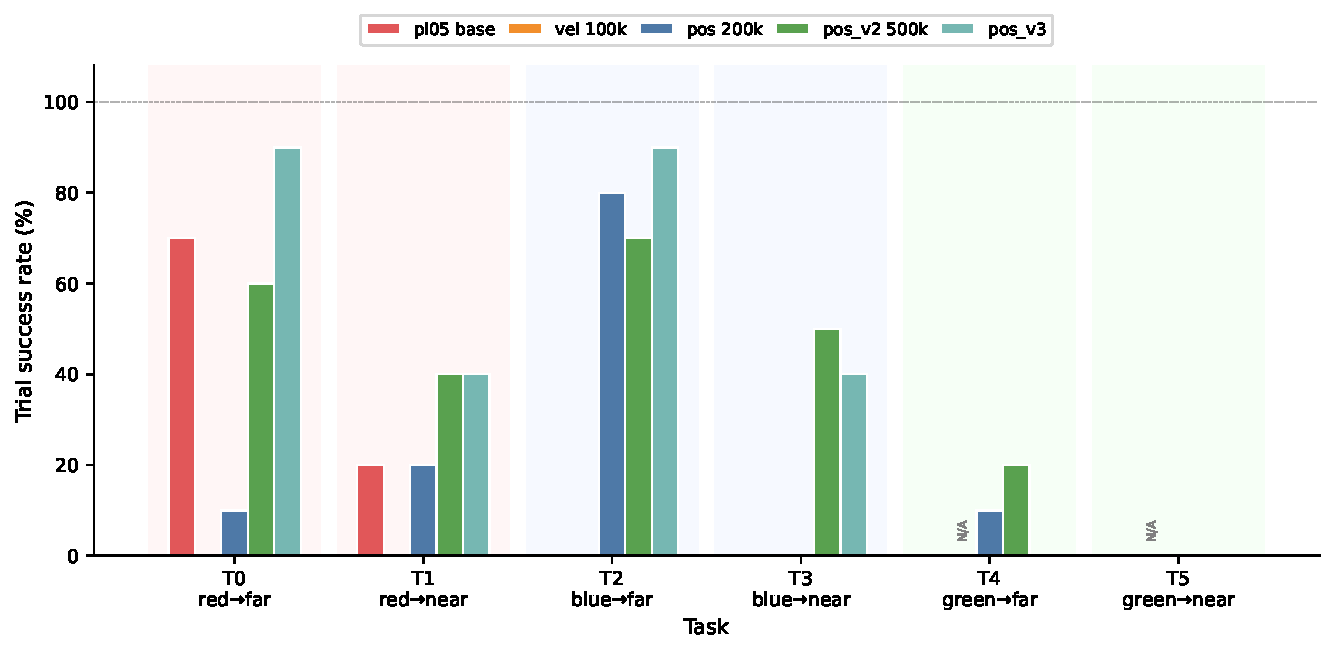
\includegraphics[width=\columnwidth]{figures/success_bar_chart.pdf}
    \caption{Per-task trial-level success rates across all five checkpoints
    (\texttt{pi05\_base}, \texttt{vel~100k}, \texttt{pos~200k},
    \texttt{pos\_v2~500k}, \texttt{pos\_v3}).
    Far-side tasks (T0, T2, T4) consistently outperform their near-side
    counterparts (T1, T3, T5) for all fine-tuned position-control checkpoints.
    Green block tasks (T4, T5) show no improvement beyond the 200k-step
    checkpoint despite additional training and demonstrations.}
    \label{fig:success_bar}
\end{figure}

\begin{figure}[t]
    \centering
    % Suggested figure: 2x3 grid of scene camera stills from a pos_v3
    \begin{tabular}{@{}ccc@{}}
        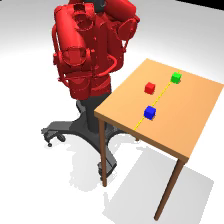
\includegraphics[width=0.31\columnwidth]{figures/exec_sequence/a_initial.png} &
        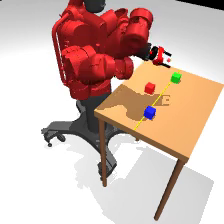
\includegraphics[width=0.31\columnwidth]{figures/exec_sequence/b_approach.png} &
        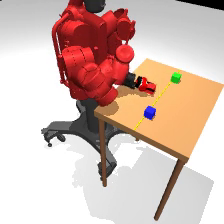
\includegraphics[width=0.31\columnwidth]{figures/exec_sequence/c_descent.png} \\
        \small (a) Initial & \small (b) Approach & \small (c) Descent \\[4pt]
        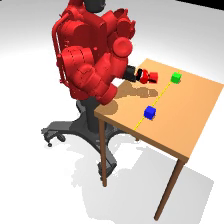
\includegraphics[width=0.31\columnwidth]{figures/exec_sequence/d_lift.png} &
        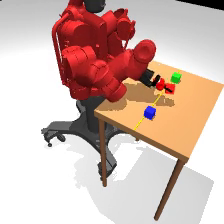
\includegraphics[width=0.31\columnwidth]{figures/exec_sequence/e_carry.png} &
        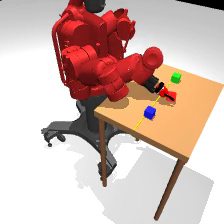
\includegraphics[width=0.31\columnwidth]{figures/exec_sequence/f_place.png} \\
        \small (d) Lift ($z{=}0.35$\,m) & \small (e) Carry ($x{=}0.75$\,m) & \small (f) Place ($x{=}0.76$\,m) \\
    \end{tabular}
    \caption{Execution sequence for a successful red-block far-side trial
    (\texttt{pos\_v3}, T0, trial~00, 9/10 success rate).
    The policy executes a complete pick-and-place sequence:
    approach, descent to within 3~mm of block centre, lift to 0.37~m,
    carry across the workspace divider, and controlled placement.
    Final block position: $x = 0.779$~m (success threshold: $x > 0.70$~m).}
    \label{fig:exec_sequence}
\end{figure}

\begin{figure}[t]
    \centering
    
\includegraphics[width=\columnwidth]{%
        /home/robotlab/Desktop/saniya_ws/pi0.5_mujoco/data/baxter/plots/06_chunk_repetition.png}
    \caption{Illustration of gripper hysteresis within a single 10-step action chunk
    (T1, \texttt{pos\_run3}, trial~00): the flow-matching denoiser produces a
    close--open--close pattern at chunk indices 7--9 (gripper\_norm values 0.53,
    0.00, 0.99). The block escapes during the transient open at index~8,
    displacing 8~mm in $x$ and 12~mm in $y$ before the gripper re-closes on air.
    The latch fix (Section~III-G) prevents this by enforcing closed state once
    gripper\_norm~$> 0.5$ until a clear placement signal (gripper\_norm~$< 0.2$).}
    \label{fig:hysteresis}
\end{figure}
